\documentclass{beamer}
\usetheme{Boadilla}

\usepackage[utf8]{inputenc}
\usepackage[T1]{fontenc}
\usepackage{amsmath}
\usepackage{pgfplots}
\pgfplotsset{compat=1.18}
\usepackage[dvipsnames,table]{xcolor}
\usepackage{tcolorbox}

\title{Aula 2}
\subtitle{Busca Binária}
\author{Maratona de Programação}
\institute{FEI}
\date{\today}

\begin{document}

\begin{frame}
	\titlepage
\end{frame}

\begin{frame}{Fundamento: Busca em Lista Ordenada}

	\textcolor{structure}{Problema}: dado um vetor A de tamanho N $(N \leq 10^6,  0 \leq A_i \leq 10^9)$ , responda Q queries $(Q \leq 10^6)$ do tipo:
	\vspace{10pt}
	\begin{center}
		\textcolor{structure}{O valor X $(X \leq 10^9)$ está presente no vetor?}

	\end{center}

\end{frame}

\begin{frame}{Fundamento: Busca em Lista Ordenada}
	\framesubtitle{Ideia de solução 1: busca completa}

	\begin{itemize}
			\pause
		\item \textcolor{structure}{Ideia:} Para cada query, olhar para o vetor A e verificar se existe algum i tal que $X == A_i$ é verdade.
			\pause
		\item Isso com certeza da o resultado certo, já que toda posição é explorada.
			\pause
		\item Por que essa solução \textcolor{red}{\textbf{não}} é ótima?
			\pause
		\item Complexidade de tempo: \textbf{$\mathcal{O}{(N*Q)}$}.
			\pause
		\item Quantidade de operacoes no pior caso: \textbf{$10^6 * 10^6 = 10^{12}$}.
			\pause
		\item Resultado: \textcolor{red}{\textbf{Time Limit Exceeded (TLE)}}.
	\end{itemize}

\end{frame}

\begin{frame}{Fundamento: Busca em Lista Ordenada}
	\framesubtitle{Ideia de solução 2: Pré-processamento}

	\begin{itemize}
			\pause
		\item \textcolor{structure}{Ideia:} Antes das queries, criar um vetor $V$ de tamanho $\max_{i = 1}^{n} A_i$, preenchido com $0$.
			\pause
		\item Para cada $A_i \in A$, fazer $V_{A_i} := 1$.
			\pause
			\vspace{10pt}

			\begin{center}
				\renewcommand{\arraystretch}{1.3}
				\setlength{\tabcolsep}{8pt}

				\begin{tabular}{c c}
					$A:$ &
					{
						\rowcolors{1}{structure!10!white}{structure!5!white}
						\begingroup
						\color{structure}
						\begin{tabular}{|c|c|c|c|c|}
							\hline
							1 & 3 & 5 & 6 & 8 \\
							\hline
						\end{tabular}
						\endgroup
					}
				\end{tabular}

				\pause
				\vspace{10pt}
				\begin{tabular}{c c}
					$V:$ &
					{
						\rowcolors{1}{structure!10!white}{structure!5!white}
						\begingroup
						\color{structure}
						\begin{tabular}{|c|c|c|c|c|c|c|c|c|}
							\hline
							0 & 1 & 0 & 1 & 0 & 1 & 1 & 0 & 1 \\
							\hline
						\end{tabular}
						\endgroup
					}
				\end{tabular}

				\vspace{-8pt}
				\begin{tabular}{c c}
					\hspace{25pt}
					\setlength{\tabcolsep}{9.3pt}
					{\tiny
					\begin{tabular}{ccccccccc}
						0 & 1 & 2 & 3 & 4 & 5 & 6 & 7 & 8 \\
					\end{tabular}
					}
				\end{tabular}
			\end{center}

			\pause
		\item Agora, eu consigo responder uma query com uma busca num vetor.
			\pause
		\item Por que essa solução \textcolor{red}{\textbf{não}} é ótima?

	\end{itemize}

\end{frame}

\begin{frame}{Fundamento: Busca em Lista Ordenada}
	\framesubtitle{Ideia de solução 2: Pré-processamento}

	\begin{itemize}
			\pause
		\item Complexidade de tempo: \textbf{$\mathcal{O}{(N + Q)}$} \pause \textcolor{green}{(OK)}.
			\pause
		\item Complexidade de espaco: \textbf{$\mathcal{O}{(\max_{i = 1}^{n} A_i)}$}.
			\pause
		\item Memoria necessaria no pior caso: \textbf{$10^9 / sizeof(bool) \approx 125MB$}.
			\pause
		\item Resultado: \\ \textcolor{red}{\textbf{Memory Limit Exceeded (MLE) ou Runtime Error (RTE)}}.
	\end{itemize}

\end{frame}

\begin{frame}{Fundamento: Busca em Lista Ordenada}
	\framesubtitle{Ideia de solução 3: Busca Binária}


	\begin{itemize}
			\pause
		\item \textcolor{structure}{Ideia:} Para cada query, buscamos o primeiro $i$ tal que $A_i \geq X$.
			\pause
		\item Começamos considerando todo o segmento \([1, N]\) como possível resposta.
			\pause
		\item Escolhemos o valor no meio do segmento e verificamos se ele é \(\geq X\).
			\pause
		\item Se for, ele pode ser uma resposta, mas ainda tentamos encontrar uma posição melhor à esquerda, olhando agora para $[1, meio]$.
			\pause
		\item Se não for, descartamos ele e toda a parte à esquerda, olhando agora para $(meio, N]$.
			\pause
		\item Repetimos até o sobrar só um valor. A posição final encontrada (se houver) é a menor com valor \(\geq X\).
	\end{itemize} 
\end{frame}

\begin{frame}{Busca em Lista Ordenada}
	\framesubtitle{Ideia de solução 3: Busca Binária}

	\begin{center}
		\textcolor{structure}{Visualização Query (X = 5):}
		\renewcommand{\arraystretch}{1.3}

		\vspace{10pt}

		\begin{tabular}{c c}
			$A:$ &
			{
				\rowcolors{1}{structure!10!white}{structure!5!white}
				\begingroup
				\color{structure}
				\begin{tabular}{|p{8pt}|p{8pt}|p{8pt}|p{10pt}|p{10pt}|p{10pt}|p{10pt}|p{10pt}|p{10pt}|}
					\hline
					{\only<1>{2}\only<2-4>{\underline{2}}\only<5>{\underline{\textbf{2}}}\only<6>{\cellcolor{white}{2}}} &
					{\only<1-3>{5}\only<4>{\textbf{5}}\only<5>{\underline{5}}\only<6>{\underline{\textbf{5}}}} &
					{\only<1-2>{9}\only<3>{\textbf{9}}\only<4>{\underline{9}}\only<5-6>{\cellcolor{white}{9}}} &
					{\only<1-3>{12}\only<4-6>{\cellcolor{white}{12}}} &
					{\only<1>{13}\only<2>{\textbf{13}}\only<3>{\underline{13}}\only<4-6>{\cellcolor{white}{13}}} &
					{\only<1-2>{17}\only<3-6>{\cellcolor{white}{17}}} &
					{\only<1-2>{20}\only<3-6>{\cellcolor{white}{20}}} &
					{\only<1-2>{25}\only<3-6>{\cellcolor{white}{25}}} &
					{\only<1>{26}\only<2>{\underline{26}}\only<3-6>{\cellcolor{white}{26}}} \\
					\hline
				\end{tabular}
				\endgroup
				}
		\end{tabular}

		\vspace{-8pt}

		\begin{tabular}{c c}
			\hspace{30pt}
			{\tiny
			\begin{tabular}{p{10pt}p{10pt}p{10pt}p{10pt}p{10pt}p{10pt}p{10pt}p{10pt}p{10pt}}
				0 & 1 & 2 & 3 & 4 & 5 & 6 & 7 & 8 \\
			\end{tabular}
			}
		\end{tabular}

	\end{center}
\end{frame}

\begin{frame}{Busca em Lista Ordenada}
	\framesubtitle{Ideia de solução 3: Busca Binária}

	\begin{center}
		\textcolor{structure}{Visualização Query (X = 21):}
		\renewcommand{\arraystretch}{1.3}

		\vspace{10pt}

		\begin{tabular}{c c}
			$A:$ &
			{
				\rowcolors{1}{structure!10!white}{structure!5!white}
				\begingroup
				\color{structure}
				\begin{tabular}{|p{8pt}|p{8pt}|p{8pt}|p{10pt}|p{10pt}|p{10pt}|p{10pt}|p{10pt}|p{10pt}|}
					\hline
					{\only<1>{2}\only<2>{\underline{2}}\only<3-5>{\cellcolor{white}{2}}} &
					{\only<1>{5}\only<2>{5}\only<3-5>{\cellcolor{white}{5}}} &
					{\only<1>{9}\only<2>{9}\only<3-5>{\cellcolor{white}{9}}} &
					{\only<1>{12}\only<2>{12}\only<3-5>{\cellcolor{white}{12}}} &
					{\only<1>{13}\only<2>{\textbf{13}}\only<3-5>{\cellcolor{white}{13}}} &
					{\only<1-2>{17}\only<3>{\underline{17}}\only<4-5>{\cellcolor{white}{17}}} &
					{\only<1-2>{20}\only<3>{\textbf{20}}\only<4-5>{\cellcolor{white}{20}}} &
					{\only<1-3>{25}\only<4-5>{\underline{\textbf{25}}}} &
					{\only<1>{26}\only<2-4>{\underline{26}}\only<5>{\cellcolor{white}{26}}} \\
					\hline
				\end{tabular}
				\endgroup
				}
		\end{tabular}

		\vspace{-8pt}

		\begin{tabular}{c c}
			\hspace{30pt}
			{\tiny
			\begin{tabular}{p{10pt}p{10pt}p{10pt}p{10pt}p{10pt}p{10pt}p{10pt}p{10pt}p{10pt}}
				1 & 2 & 3 & 4 & 5 & 6 & 7 & 8 & 9 \\
			\end{tabular}
			}
		\end{tabular}

	\end{center}
\end{frame}

\begin{frame}{Busca em Lista Ordenada}
	\framesubtitle{Ideia de solução 3: Busca Binária}

	\begin{center}
		\textcolor{structure}{Implementando: }\href{https://codeforces.com/edu/course/2/lesson/6/1/practice/contest/283911/problem/A}{A. Binary Search}.

	\end{center}
\end{frame}

\begin{frame}{Ponderando}
	\begin{itemize}
			\pause
		\item Qual a complexidade de tempo desse algoritmo? \pause \textbf{$\mathcal{O}{(logN)}$}.
			\pause
		\item Qual a complexidade de espaço desse algoritmo? \pause \textbf{$\mathcal{O}{(N)}$}.
			\pause
		\item \textcolor{structure}{Por que ele sempre funciona?}
	\end{itemize}
\end{frame}

\begin{frame}{Generalizando: \textbf{Monotonicidade}}
	\begin{itemize}
			\pause
		\item Se criassemos um vetor $R$, de tamanho N, tal que $R_i := A_i \geq X$, teríamos:
			\pause

			\begin{center}
				\renewcommand{\arraystretch}{1.3}

				\vspace{10pt}
				\begin{tabular}{c c}
					$A:$ &
					{
						\rowcolors{1}{structure!10!white}{structure!5!white}
						\begingroup
						\color{structure}
						\begin{tabular}{|p{8pt}|p{8pt}|p{8pt}|p{10pt}|p{10pt}|p{10pt}|p{10pt}|p{10pt}|p{10pt}|}
							\hline
							2 & 5 & 9 & 12 & 13 & 17 & 20 & 25 & 26 \\
							\hline
						\end{tabular}
						\endgroup
					}
				\end{tabular}

				\vspace{-8pt}
				\begin{tabular}{c c}
					\hspace{30pt}
					{\tiny
					\begin{tabular}{p{10pt}p{10pt}p{10pt}p{10pt}p{10pt}p{10pt}p{10pt}p{10pt}p{10pt}}
						1 & 2 & 3 & 4 & 5 & 6 & 7 & 8 & 9 \\
					\end{tabular}
					}
				\end{tabular}

				\pause
				\vspace{5pt}
				\textcolor{structure}{$X = 12$} \\ 
				\vspace{5pt}
				\begin{tabular}{c c}
					$R:$ &
					{
						\rowcolors{1}{structure!10!white}{structure!5!white}
						\begingroup
						\color{structure}
						\begin{tabular}{|p{8pt}|p{8pt}|p{8pt}|p{10pt}|p{10pt}|p{10pt}|p{10pt}|p{10pt}|p{10pt}|}
							\hline
							0 & 0 & 0 & 1 & 1 & 1 & 1 & 1 & 1 \\
							\hline
						\end{tabular}
						\endgroup
					}
				\end{tabular}

				\vspace{-8pt}
				\begin{tabular}{c c}
					\hspace{30pt}
					{\tiny
					\begin{tabular}{p{10pt}p{10pt}p{10pt}p{10pt}p{10pt}p{10pt}p{10pt}p{10pt}p{10pt}}
						1 & 2 & 3 & 4 & 5 & 6 & 7 & 8 & 9 \\
					\end{tabular}
					}
				\end{tabular}
			\end{center}

			\pause 
		\item E esse padrão para o vetor R (prefixo contendo apenas $0s$, sufixo contendo apenas $1s$) seria encontrado para todo $X$ em qualquer vetor $A$ ordenado de maneira não decrescente.

	\end{itemize}
\end{frame}

\begin{frame}{Generalizando: \textbf{Monotonicidade}}
	\begin{itemize}
		\item Isso porque, num array ordenado, nenhum valor anterior à mim vai ser maior que um valor que eu não sou maior.
			\pause
			\begin{center}
				\begin{tcolorbox}[
						colback=structure!10,
						colframe=structure,
						coltext=black,
						boxrule=1pt,
						arc=8pt,
						width=0.6\textwidth,
						enhanced,
					]
					Formalmente, basta garantir que:  \begin{center}\\ $A_i \geq A_{i-1} \forall i \in [2, N]$\end{center}\\
						Para que o vetor $R$ se pareça assim

				\end{tcolorbox}
			\end{center}

			\pause
		\item O que é sempre verdade em um vetor ordenado. Mas também é sempre verdade pra qualquer \textbf{função monotônica}.
	\end{itemize}
\end{frame}

\begin{frame}{Generalizando: \textbf{Monotonicidade}}
	\textcolor{structure}{Exemplo: $\mathcal{}{(x)} = \lfloor x \rfloor$}
	\begin{center}
		\begin{tikzpicture}
			\begin{axis}[ width=10cm, height=7cm, grid=both, xmin=0, xmax=10, ymin=0, ymax=10, domain=0:10, samples=21, axis lines=middle, xlabel={$x$}, ylabel={$f(x)$}, ]
				\addplot[red, thick, mark=none, const left] {floor(x)};
			\end{axis}
		\end{tikzpicture}
	\end{center}
\end{frame}

\begin{frame}{Generalizando: \textbf{Monotonicidade}}
	\textcolor{structure}{Exemplo: $\mathcal{f}{(x)} = \frac{x(x - 1)}{2}$}
	\begin{center}
		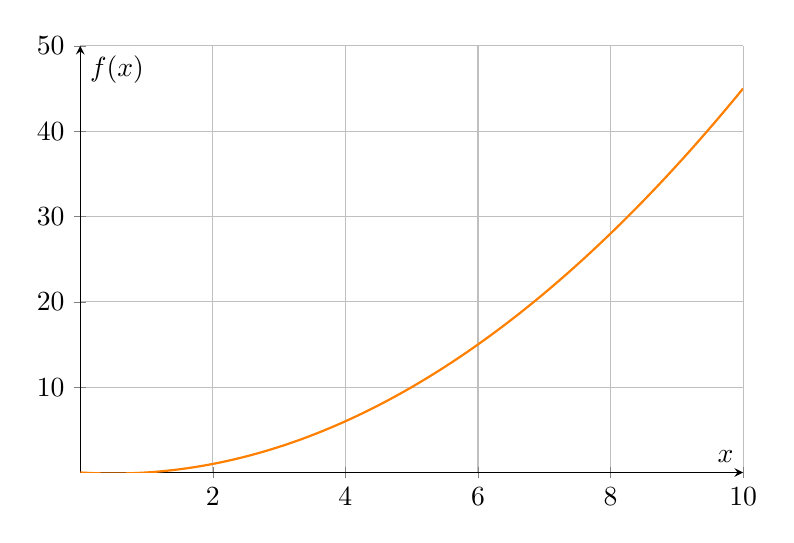
\begin{tikzpicture}
			\begin{axis}[ width=10cm, height=7cm, grid=both, xmin=0, xmax=10, ymin=0, ymax=50, domain=0:10, samples=200, axis lines=middle, xlabel={$x$}, ylabel={$f(x)$}, ]
				\addplot[orange, thick] {x*(x - 1)/2};
			\end{axis}
		\end{tikzpicture}
	\end{center}
\end{frame}

\begin{frame}{Generalizando: \textbf{Monotonicidade}}
	\textcolor{structure}{Exemplo: $\mathcal{f}{(x)} = \max\left(1, \frac{(x - 5)^3}{3} + x\right) + 2(\lfloor \frac{x}{2} \rfloor)$}
	\begin{center}
		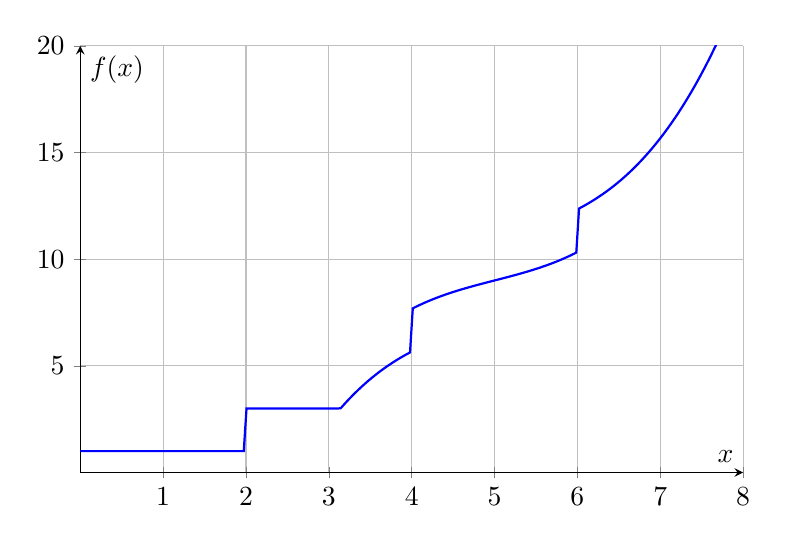
\begin{tikzpicture}
			\begin{axis}[ width=10cm, height=7cm, grid=both, xmin=0, xmax=8, ymin=0, ymax=20, domain=0:10, samples=300, axis lines=middle, xlabel={$x$}, ylabel={$f(x)$}, ]
				\addplot[blue, thick] {max(1, (x - 5)^3/3 + x) + floor(x / 2) * 2};
			\end{axis}
		\end{tikzpicture}
	\end{center}
\end{frame}

\begin{frame}{Busca binária na maratona}
	\begin{itemize}
		\item Resumindo: 
			\pause
			\begin{center}
				\begin{tcolorbox}[
						colback=structure!10,
						colframe=structure,
						coltext=black,
						boxrule=1pt,
						arc=8pt,
						width=0.75\textwidth,
						enhanced,
					]
					Para qualquer problema de maratona, é possível achar:
					\begin{itemize}
						\item Primeiro ponto tal que $\mathcal{f}{(x)} \leq Y$ ou,
						\item Último ponto tal que $\mathcal{f}{(x)} > Y$ ou,
						\item qualquer outra variação de condição que faça o vetor $R$ parecer com: $R = [0, 0, 0, 1, 1, 1, 1]$.
					\end{itemize}
				\end{tcolorbox}
			\end{center}
			\pause
		\item Algumas pessoas chamam essa ideia de "busca binária na resposta".
			\pause
		\item A dificuldade dos problemas usualmente é:
			\begin{itemize}
					\pause
				\item Notar que uma	$\mathcal{f}{(x)}$, útil para resolver o problema, é monotônica.
					\pause
				\item Achar um jeito esperto de computar $\mathcal{f}{(x)}$.
			\end{itemize}

	\end{itemize}
\end{frame}

\begin{frame}{Busca binária na maratona}
	\framesubtitle{Exemplo resolvido 1:}

	\begin{center}
		\textcolor{structure}{BeeCrowd: }\href{https://judge.beecrowd.com/pt/problems/view/3420}{Torre de Cartas}.
	\end{center}
\end{frame}

\begin{frame}{Busca binária na maratona}
	\framesubtitle{Exemplo resolvido 2:}

	\begin{center}
		\textcolor{structure}{CSES: }\href{https://cses.fi/problemset/task/1085}{Array Division}.
	\end{center}
\end{frame}

\begin{frame}{Busca binária na maratona}
	\framesubtitle{Exemplo comentado 1:}

	\begin{center}
		\textcolor{structure}{CodeForces: }\href{https://codeforces.com/contest/782/problem/B}{B. The Meeting Place Cannot Be Changed}.
	\end{center}
\end{frame}

\begin{frame}{Busca binária na maratona}
	\framesubtitle{Exemplo comentado 2:}

	\begin{center}
		\textcolor{structure}{CodeForces: }\href{https://codeforces.com/group/KqUNBZJnMk/contest/584381/problem/K}{K. Delivery Bears}.
	\end{center}
\end{frame}

\begin{frame}{Listas de problemas relacionados}
	\framesubtitle{Lista conhecidas:}

	\begin{itemize}
		\item \textcolor{structure}{UFMG: \textbf{\href{https://docs.google.com/spreadsheets/d/1QQ1QvYNDPKv9Aqh5c2VL_KCtpqASDWeRcLkyyXlPM0M/edit?gid=1907459156#gid=1907459156}{link}}. }
			\begin{itemize}
				\item veja também o vídeo deles \textcolor{structure}{\textbf{\href{https://www.youtube.com/watch?v=s9W9zJrcrzY}{aqui}}}.
			\end{itemize}
		\item \textcolor{structure}{USACO Guide: \textbf{\href{https://usaco.guide/silver/binary-search}{link}}. }
		\item \textcolor{structure}{UTL: \textbf{\href{https://youkn0wwho.academy/topic-list/binary_search}{link}}. }
	\end{itemize}
\end{frame}

\end{document}
